\documentclass{article}
\usepackage{amsmath}
\usepackage{pgfplots}

\title{Differential Equations Homework 02}
\author{Your Name}
\date{}

\begin{document}

\maketitle

\section*{Problem 1(b)}

The given ODE is \( y' = 2y - y^2 \). We need to sketch the direction field for \( -3 \leq t \leq 3 \) and \( -3 \leq y \leq 3 \).

\subsection*{Direction Field}

The direction field is created by plotting small line segments with slope equal to \( y' = 2y - y^2 \) at various points in the region. Below is the direction field with a solution passing through the point \( (0,1) \).

\begin{figure}[h!]
    \centering
    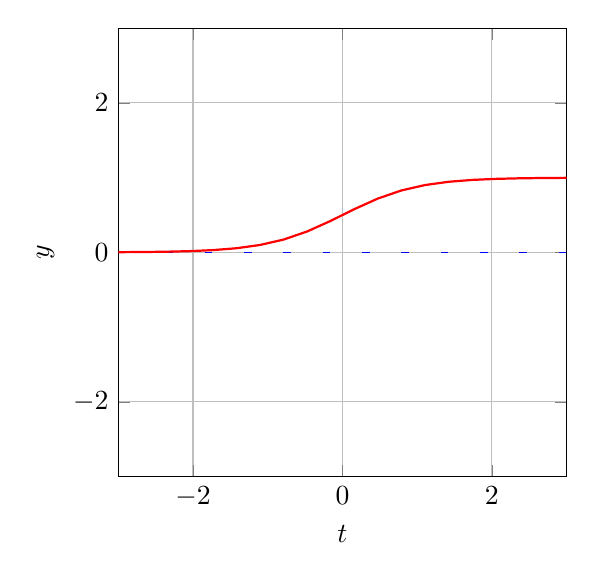
\begin{tikzpicture}
        \begin{axis}[
            xlabel={$t$},
            ylabel={$y$},
            axis equal image,
            grid=major,
            xmin=-3, xmax=3,
            ymin=-3, ymax=3,
            samples=20
            ]
        \addplot[quiver={
            u={1}, v={2*y - y^2},
            scale arrows=.1
        }, blue] {0};
        \addplot[domain=-3:3, red, thick] {1/(1 + e^(-2*x))}; % Example solution curve
        \end{axis}
    \end{tikzpicture}
    \caption{Direction field for \( y' = 2y - y^2 \) and solution curve passing through \( (0, 1) \).}
\end{figure}

\end{document}
